\section{Accuracy}
\label{sec:accuracy}
 
One of the most reliable way to assess the simulation's accuracy at evolving particles
is to measure the density power spectrum at late time, and compare to non-linear prediction. 
For an over-density field $\delta({\bf \it x})$, the power spectrum is extracted from the two point function in Fourier space as:
\begin{eqnarray}
\langle | \delta ({\bf \it k}) \delta ({\bf \it k'}) | \rangle = (2\pi)^{3}P(k)\delta_{D}({\bf \it k'} - {\bf \it k})
\label{eq:power}
\end{eqnarray}
where the angle bracket corresponds to an ensemble (or volume) average.
We plot in Fig. \ref{fig:power_highres} the dimensionless power spectrum for a large run ($4000^3$ particles),
which are evolved from a Gaussian initial distribution at $z=100$ down to $z=0$, in a box $3.2 h^{-1}\mbox{Gpc}$ per side.
We observe that the agreement with the non-linear prediction of \cite{Lewis:1999bs} is at the per cent level over a large dynamical range.
The drop of power at high-$k$ is caused by the finite resolution, and the fluctuations at low-$k$ is caused by the white noise imposed
in the initial conditions. 

\begin{figure*}%[ht]
  \begin{center}
    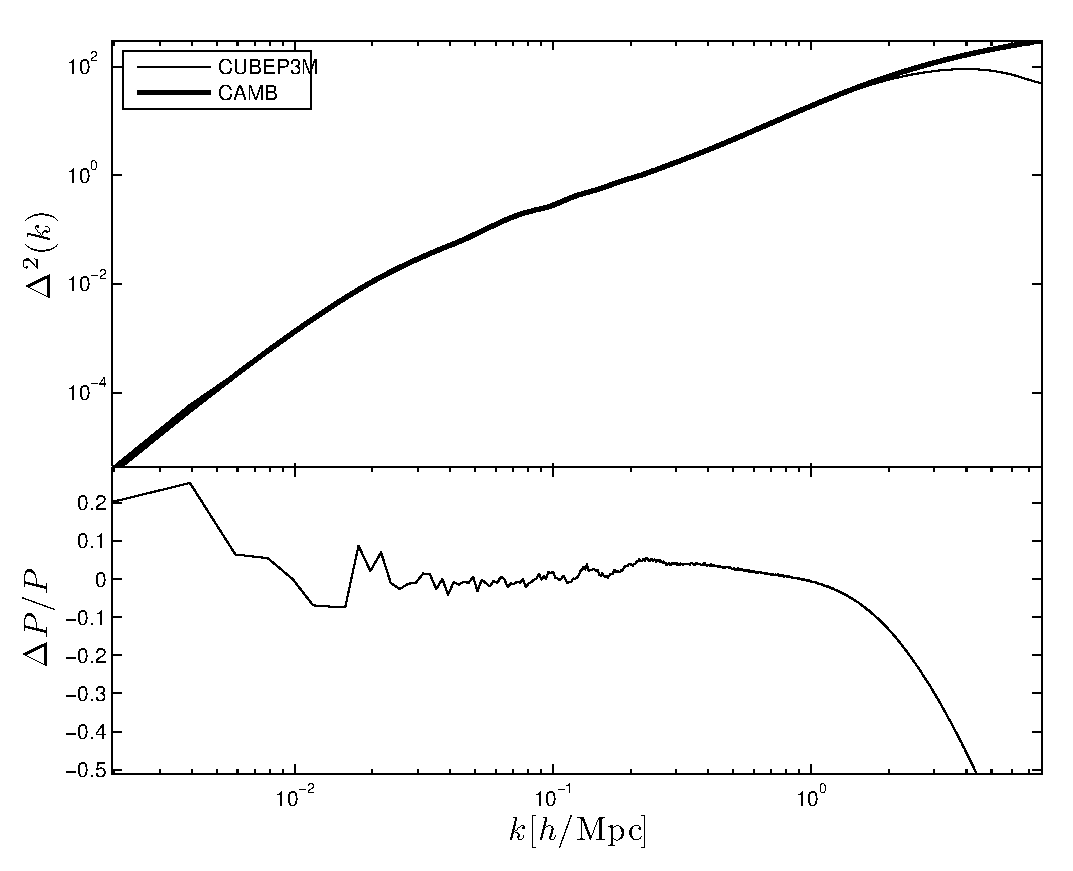
\includegraphics[width=5.2in]{graphs/power_highres.eps}
  \caption{Dark matter power spectrum, measured at $z=0$ in a volume $3.2 h^{-1}\mbox{Gpc}$ per side,
  from $4000^3$ particles. The simulation ran on 4000 cores on Ranger.
    \label{fig:power_highres}}
\end{center}
\end{figure*}

The actual force of gravity on the p$^3$m algorithm is presented in Fig. \ref{fig:den_force_ppext0}.
This is a force versus distance plot, where the force is calculated in two steps. 
We first compute the force on each particles of a given distribution as done at every time step.
We then remove one particle, compute the force again on all particles, and record on a file the 
force difference between the two calculations and the distance to the `hole'.

Fig. \ref{fig:den_force_fracErr} shows the fractional error on the force along the radial and tangential directions.
It is larger than in {\small PMFAST} at grid scales, largely due to the fact that the fine mesh force is performed with an NGP interpolation scheme -- as opposed to CIC -- which shows a larger scatter about the theoretical value. {\bf (I would like to mention why we opted for NGP. Can't we do p3m with CIC on the fine grid? )}


\begin{figure}%[ht]
  \begin{center}
    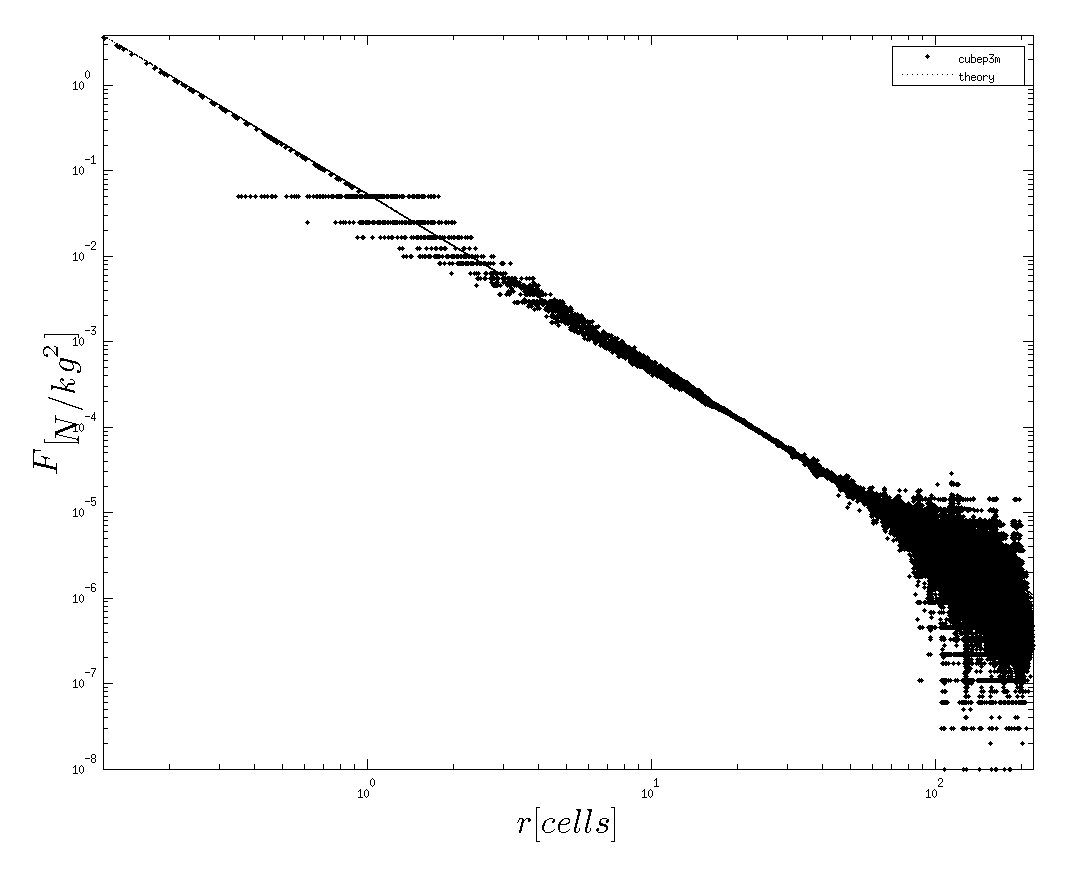
\includegraphics[width=3.2in]{graphs/densityForce_ppext=0.eps}
  \caption{Gravity force in of the p$^3$m algorithm, versus distance in fine mesh cell units, compared with the exact $1/r^{2}$ law.
  Particles in the same fine cell follow the exact curve, then we observe a large scatter at 
  distance of the order of the fine grid, caused by the NGP interpolation scheme. 
    \label{fig:den_force_ppext0}}
\end{center}
\end{figure}

\begin{figure}%[ht]
  \begin{center}
    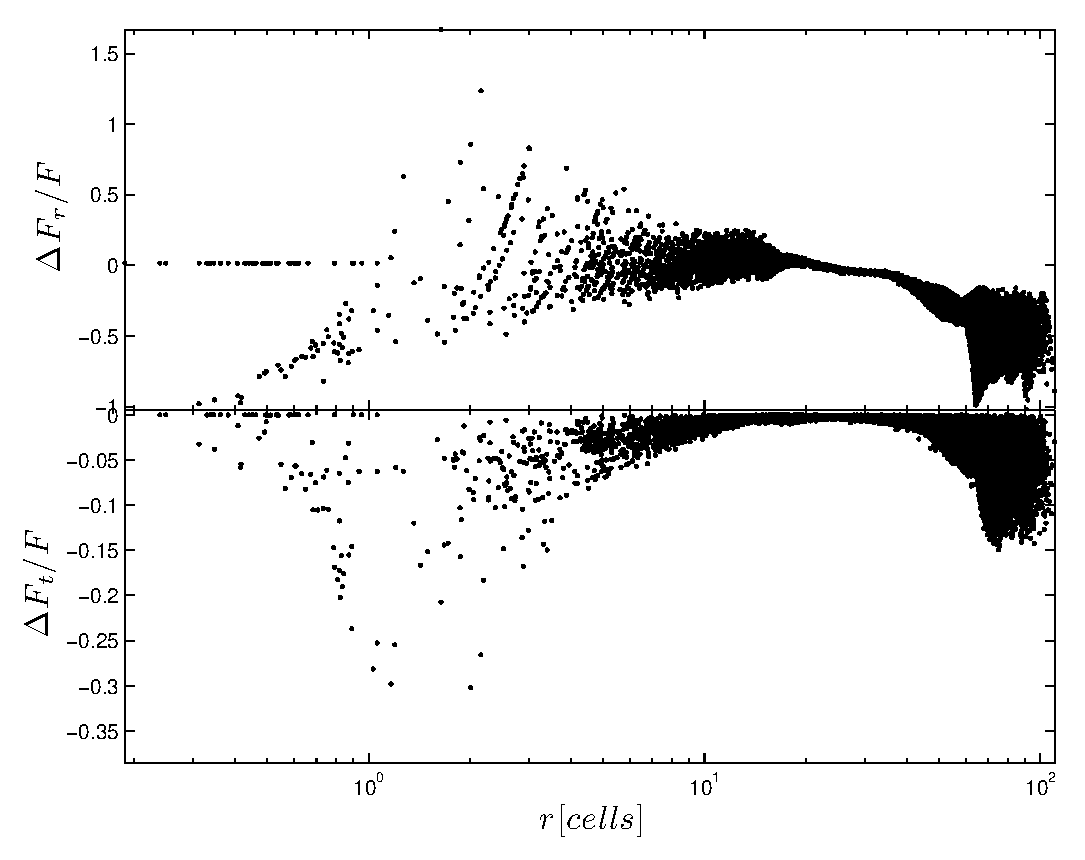
\includegraphics[width=3.2in]{graphs/densityForce_fracErr.eps}
  \caption{Fractional error on the force in of the p$^3$m algorithm, in the radial (top) and tangential(bottom) directions.
    \label{fig:den_force_fracErr}}
\end{center}
\end{figure}


\section{Systematics}
\label{sec:systematics}

\subsection{Mesh force at grid distances}

The biggest problem with the pp force calculation is that it 
is anisotropic and depends on the location of the fine mesh with respect 
to the particles. An example are two particles on either side of a grid 
cell boundary. These particles will experience the 1-grid cell separation
NGP mesh force, but if the mesh were shifted such that they were
within the same cell, they would experience the (larger) pp force instead. 
This effect is especially pronounced at the early stages of the simulation where
the density is more homogeneous, and leads to mesh artefacts appearing
in the density field. In order to minimize this systematic effect, 
we randomly shift the particle distribution relative to the mesh by a small
amount -- up to 2 fine grid cells in magnitude -- in each
dimension and at each time step.  This adds negligible computational
overhead as it can be applied during the particle position update
and suppresses the mesh behaviour over multiple time steps.
It is possible to shift back the particles at the end of each time steps,
which prevents a random drift of the whole population.
This is convenient if one needs to correlate the initial and final positions of the particles.
 
We ensure that, on average, this solution balances out the mesh feature,
by tuning the NGP force kernel such as to provide  force as unbalanced as possible at grid cell distances.
This adjustment is performed from the pairwise force test described in section \ref{sec:accuracy}.
We note that this is one of the driving argument to extend the pp force outside the fine mesh cell,
since the scattering of the NGP force about the actual $1/r^{2}$ law drops rapidly as the distance increases.
As discussed in section \ref{subsec:extendedpp}, this gain in accuracy comes at a price,
a choice that  must be carefully balanced.

\subsection{Constraining redshift jumps}

At early stages of the simulation, the density fields is rather homogenous, causing the force of gravity to be
rather weak everywhere. In that case, the size of the redshift jumps is controlled by a limit in the cosmological expansion.
If the expansion jump is too large, the size of the residual errors can become significant, and one can observe, for instance,
a growth of structure that does not match the predictions of  linear theory even at the largest scales.
One therefore needs to choose a maximum step size. In {\small CUBEP3M}, this is controlled by $r_{max}$, which is the fractional step size,
$\mbox{d}a/(a + \mbox{d}a)$ and is set to 0.05 by default.  Generally, a simulation should start at a redshift high enough that
the initial dimensionless power spectrum is well under unity at all scales. This ensures that the Zel'dovich approximation
 holds at the pre cent level at least. A drop of accuracy can occur if one starts the simulation too early, where
 truncation error will be significant at the early time steps.


It is possible to reduce this effect, and thereby improve significantly 
the accuracy of the code, by modifying the value of $r_{max}$, at the cost of increasing the total number of time steps.
Fig. \ref{fig:ra_max} shows a comparison of late time power spectra of density fields that originate from the same initial conditions, and used the same random seeds to control the fine mesh shifts (mentioned above), but the value of $r_{max}$ was modified at each run. 
We observe that the impact is mostly located in the non-linear regime, where decreasing the time step to 0.006 
allows the simulation to recover about 30 per cent of dimensionless power at the turn over scale, in this simulation configuration.
This gain is greatly affected by the choice of initial redshift, the resolution, and the box size, and ideally one would make
test runs in order to optimize a given configuration.  
As expected, the {\small CPU} resources required to run these simulations increase rapidly as $r_{max}$ decreases, as seen in Table \ref{table:ra_max}. 
In this test case, reducing further at 0.001 shows only a mild improvement in accuracy, but the gain in time is more than a factor of four.


\begin{figure}%[ht]
  \begin{center}
    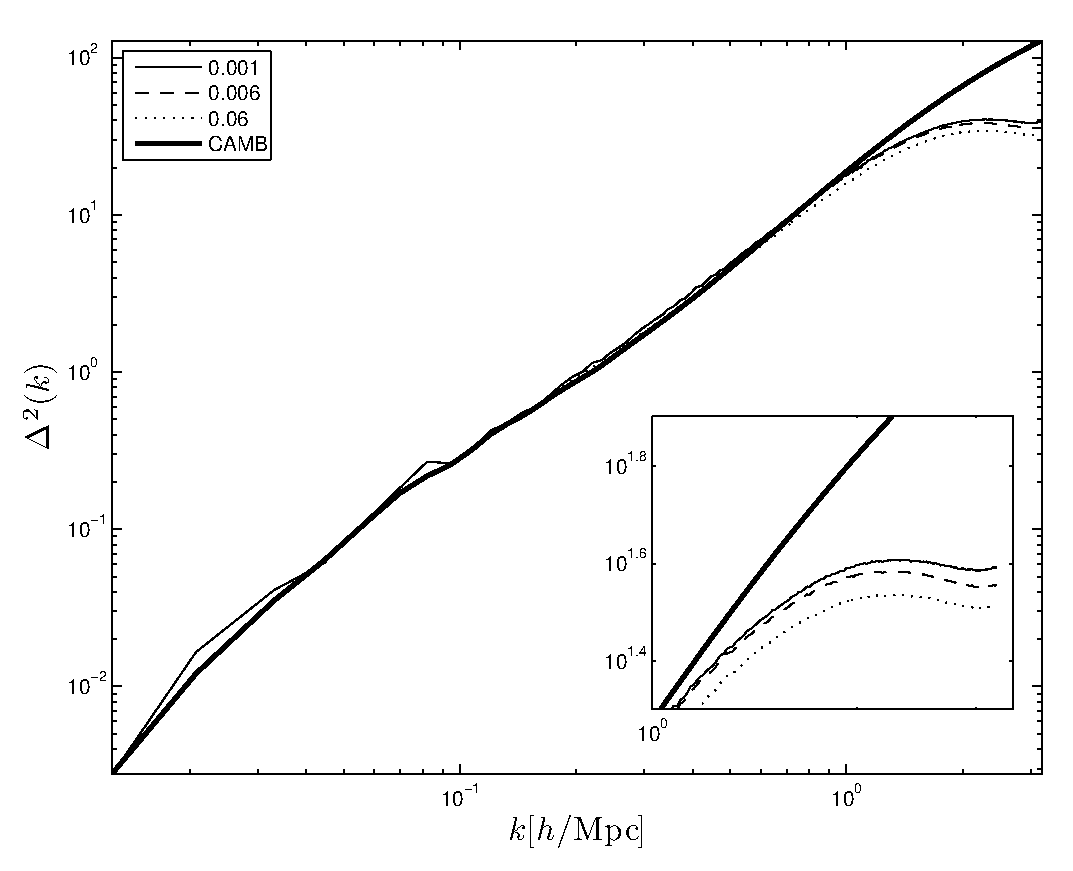
\includegraphics[width=3.2in]{graphs/power_ra_max.eps}
  \caption{Dark matter power spectrum, measured at $z=0$ in a volume $500 h^{-1}\mbox{Mpc}$ per side,
  from $256^3$ particles and a starting redshift of $z=200$. The different curves show different values of $r_{max}$. 
  The resources required to run these simulations increase rapidly as $r_{max}$ decreases.    \label{fig:ra_max}}
\end{center}
\end{figure}

\begin{table}
\begin{center}
\caption{Scaling in {\small CPU} resources as a function of the value of $r_{max}$. The tests were performed 
on the CITA Sunnyvale cluster, and general trends could vary slightly on other machines.}
\begin{tabular}{|l|c|c|}
\hline 
$r_{max}$         & time (h)   \\                 
\hline
 $0.1$ & 1.46 \\
 $0.06$ & 1.48\\
 $0.01$ & 1.67 \\
 $0.006$ & 1.91\\
 $0.003$ & 2.83 \\
 $0.002$ & 4.13\\
 $0.001$ & 8.15\\
\hline
\end{tabular}
\label{table:ra_max}
\end{center}
\end{table}


{\bf (Any other systematics effects we want to discuss here?)}

 


